\begin{frame}{What do we need?}
\begin{itemize}
    \item We need a model that can:
    \begin{itemize}
        \item \textbf{Find Patterns in Images}: Recognize small features like edges and shapes in different parts of the image.
        \item \textbf{Work Efficiently}: Avoid looking at every pixel separately by focusing on groups of pixels together.
        \item \textbf{Handle Changes}: Still recognize the same object even if it moves, rotates, or looks slightly different.
    \end{itemize}
\end{itemize}
\end{frame}

\begin{frame}{What do we need?}
\begin{itemize}
    \item We need a model that can:
    \begin{itemize}
        \item \textbf{Find Patterns in Images}: Recognize small features like edges and shapes in different parts of the image.
        \item \textbf{Work Efficiently}: Avoid looking at every pixel separately by focusing on groups of pixels together.
        \item \textbf{Handle Changes}: Still recognize the same object even if it moves, rotates, or looks slightly different.
        \item We need \textbf{Convolutional Neural Networks (CNNs)!}
    \end{itemize}
\end{itemize}
\end{frame}

\begin{frame}{Convolutional Neural Networks (CNNs)}
\begin{itemize}
        \item CNNs are neural networks designed for image processing and consist of two main parts:
        \begin{itemize}
            \item \textbf{Feature Extractor}: Automatically learns patterns (features) such as edges, textures, and shapes from the image.
            \item \textbf{Classifier}: The extracted features are flattened into a vector and passed to a standard neural network (like the ones we used before) for classification.
    \end{itemize}
\end{itemize}

\begin{figure}
        \centering
        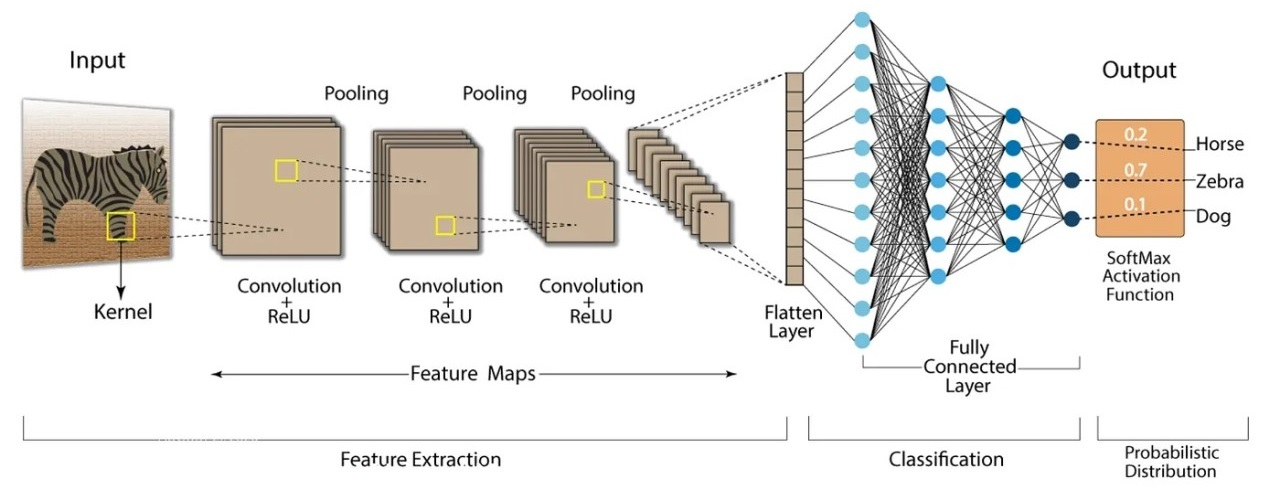
\includegraphics[width=0.9\textwidth,height=0.7\textheight,keepaspectratio]{images/cnn/cnn-fully-connected.jpeg}
        \caption{Convolutional Neural Network}
\end{figure}
\end{frame}

\begin{frame}{Convolutional Neural Networks (CNNs)}
\begin{itemize}
    \item The feature extractor consists of three essential components:
    \begin{itemize}
        \item \textbf{Convolution Layers}: Detect local patterns such as edges, textures, and shapes by applying filters to the image.
        \item \textbf{Activation Function (ReLU)}: Adds non-linearity.
        \item \textbf{Pooling Layers}: Reduce the spatial size of extracted features.
    \end{itemize}
    \item Let's start with the convolution layer.
\end{itemize}
\end{frame}

\begin{frame}{Components of a CNN}
\begin{figure}
\centering
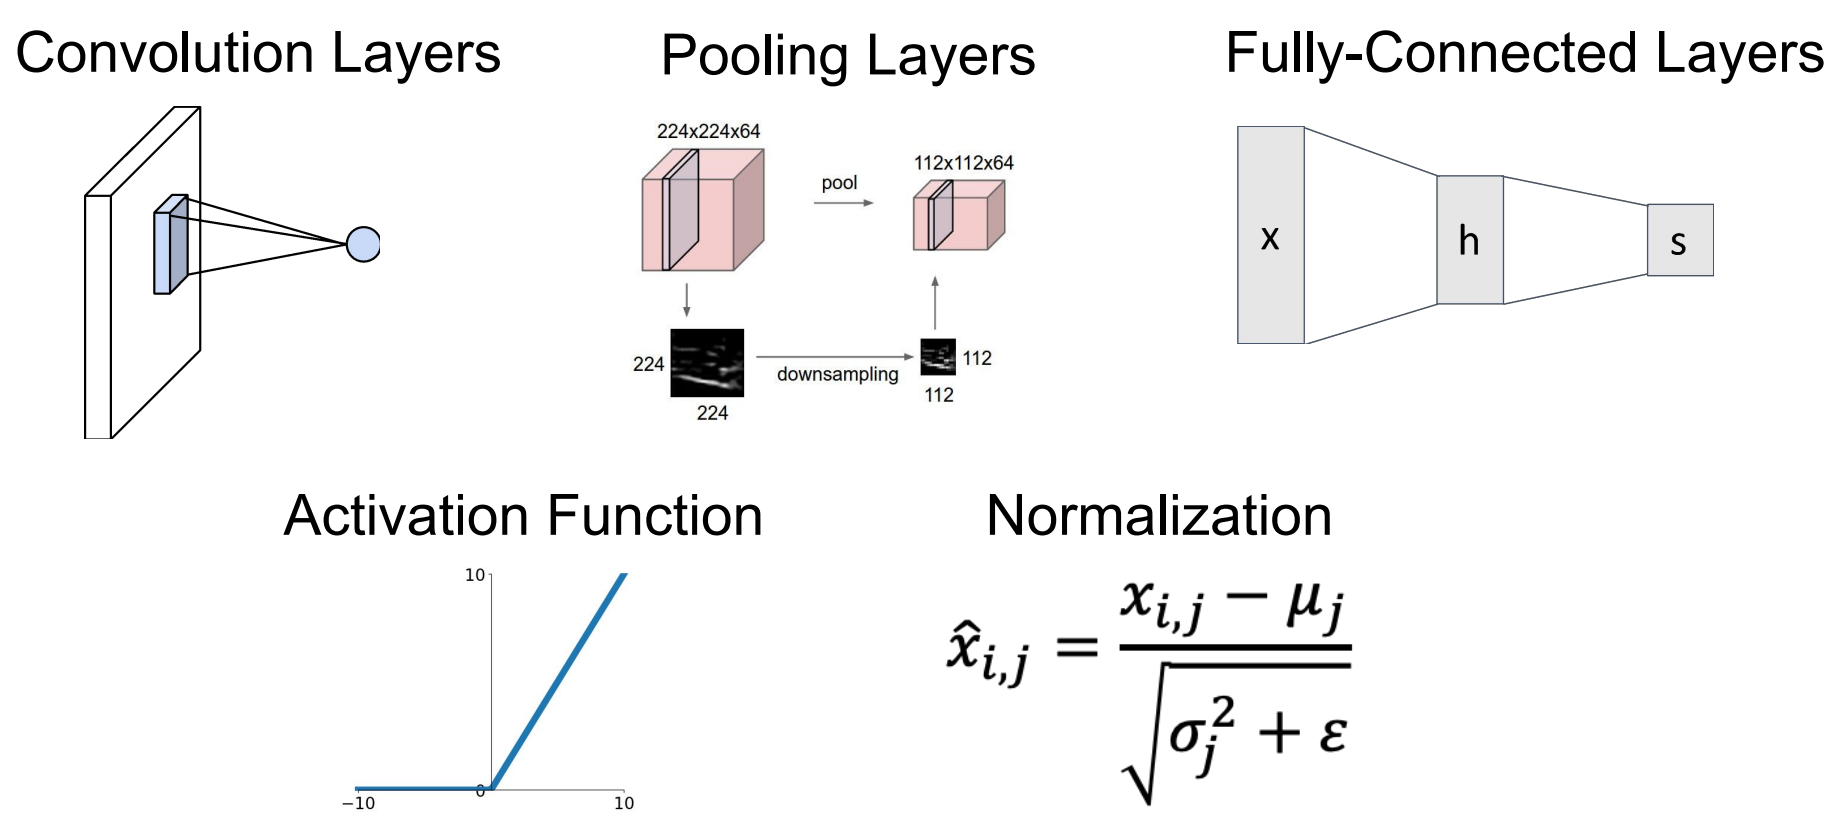
\includegraphics[width=1.0\textwidth,height=0.9\textheight,keepaspectratio]{images/cv-intro/components.png}
\end{figure}
\end{frame}
